\chapter{BLAST-TNG LEKID Readout Operator's Manual}\label{mcp}

\section{Glossary of Terms}

\noindent
\textbf{1GbE}: One-gigabit-per-second ethernet interface. Maximum bitrate is significantly less than 1 Gbps.\\
\textbf{ADC}: Also: A/D. Analog-to-digital-converter.\\
\textbf{Attenuator server}: A TCP server running in the background on each Pi. The TCP server is created by a Python script, \texttt{rudat\_server\_boot.py}, which runs in background on each Pi. MCP is the client for the server (see: \texttt{roach.c}, \texttt{atten\_client()}). See also: RUDAT.\\
\textbf{Baseband}: Also: Complex baseband. A frequency spectrum centered at 0 Hz. This is also the band which is synthesized/digitized by the digital electronics (MUSIC board and FPGA). It spans -256 to +256 MHz (512 MHz total). Each baseband frequency has a corresponding RF carrier frequency (see: probe tone).\\
\textbf{BORPH}: The Berkeley Operating System for Reprogrammable Hardware. A Linux-based operating system running on the PPCs. See: \href{https://casper.ssl.berkeley.edu/wiki/BORPH}{BORPH}\\
\textbf{CASPER}: The Collaboration for Astronomical Signal Processing and Electronics Research. See: \href{https://casper.berkeley.edu}{CASPER}\\
\textbf{Channel}: A unique detector timestream, containing the 32b I and 32b Q values for a single resonator on the array, sampled at 488.28125 Hz. Channel values are saved to disk. Each channel number maps to a single baseband/RF frequency pair. Channel numbers are zero-indexed, and increment in baseband frequency order, i.e., channel 10 corresponds to the 10th baseband frequency in the list of baseband frequencies (e.g., \texttt{bb\_target\_freqs.dat}).\\
\textbf{DAC}: Also: D/A. Digital-to-analog-converter.\\
\textbf{Demodulator}: Also: Downconverter. Polyphase AD0540B. A quadrature mixer used to downconvert RF/IF to baseband I and Q. There is one in each ROACH slice.\\
Inputs:
\setlist[description]{leftmargin=\parindent,labelindent=\parindent,nosep}
\begin{description}
  \item[$\bullet$] RF signal from the cryostat, containing the multiplexed waveforms from each pixel. LO signal generated by the Valon Synthesizer. The default LO frequency is 750 MHz (i.e., on system restart).
\end{description}
Outputs:
\setlist[description]{leftmargin=\parindent,labelindent=\parindent,nosep}
\begin{description}
  \item[$\bullet$] Baseband I and Q.
  \item[$\bullet$] Power: +5 and -5 VDC, fed by Vicor DC/DC converter in Roach box.
\end{description}
\href{https://polyphasemicrowave.com/media/AD0540B.pdf}{Datasheet: Polyphase AD0540B}\\
\textbf{df}: ‘delta-f’. The amount in Hz by which a channel’s resonant (not carrier) frequency has drifted. In the ideal, linear operational regime, df is inversely proportional to the amount of absorbed power in a channel.\\
\textbf{Downconverter}: See Demodulator. \\
\textbf{fpg}: A CASPER firmware bitstream file type. Unlike a typical .bit file, an fpg contains ASCII-formatted metadata about its contents, which is inserted at the end of the binary data. The ROACH FPGA firmware is located on FC1 and FC2 at: /data/etc/blast/roachFirmware\\
\textbf{FPGA}: Field Programmable Gate Array. A reprogrammable integrated-circuit found on each ROACH-2 board, which runs the ASU open-source KID readout firmware. The FPGAs perform the real-time digital signal processing which is necessary to readout the BLAST detectors. These particular FPGAs are Xilinx Virtex-6 models.\\
\textbf{I}: The In-phase (real, cosine) component of a complex waveform.\\
\textbf{IF}: Intermediate-frequency. The frequency spectrum produced by mixing baseband frequencies with the LO. In BLAST-TNG, IF coincides with RF, which is roughly 284--1056 MHz.\\
\textbf{KATCP}: The Karoo Array Telescope Protocol. A KATCP server running on each ROACH PPC provides I/O access to the FPGA firmware registers, as well as to a basic set of commands which can be used to query and control the PPC.\\
See: \href{https://casper.ssl.berkeley.edu/wiki/KATCP}{KATCP}\\
\textbf{LEKID}: Also, KID. Lumped Element Kinetic Inductance Detector.\\
\textbf{LO}: A variable tone produced by the Valon Synthesizer, and used to up/downconvert baseband to IF/RF in the mod/demodulators. On system start, each of the LOs are set to 750 MHz. During normal operation, the LOs remain at the center frequencies of each detector array. During sweeps, they are moved. The LO frequencies can be set and read by command (see: LO commands).\\
LO center frequencies for each array:
\setlist[description]{leftmargin=\parindent,labelindent=\parindent,nosep}
\begin{description}
  \item[$\bullet$] 500 (ROACH1): 540 MHz
  \item[$\bullet$] 250U (ROACH2): 827 MHz
  \item[$\bullet$] 250W (ROACH5): 828 MHz
% \item[$\bullet$] 350 (ROACH3): 850 MHz
\end{description}
\textbf{LUT}: Look-up-table.\\
\textbf{MKID}: Also, KID. Microwave Kinetic Inductance Detector.\\
\textbf{MODULATOR}: See Upconverter. Polyphase Microwave AM0350A. A quadrature mixer used to upconvert baseband I and Q to IF/RF I and Q. There is one in each ROACH slice.\\
Inputs:
\setlist[description]{leftmargin=\parindent,labelindent=\parindent,nosep}
\begin{description}
  \item[$\bullet$] Baseband I and Q, synthesized by the MUSIC board I and Q DACs.
  \item[$\bullet$] LO signal generated by the Valon Synthesizer. The default LO frequency is 750 MHz (i.e., on system restart).
  \item[$\bullet$ ]IF/RF signal which is sent to the cryostat.
  \item[$\bullet$] Power: +5 and -5 VDC, fed by Vicor DC/DC converter in Roach box.
\end{description}
See: \href{https://polyphasemicrowave.com/media/AM0350A_RevA.pdf}{Datasheet: Polyphase AM0350A}\\
\textbf{MUSIC Board}: A DAC/ADC board originally developed for the MUSIC camera (Multi-color Sub-millimeter Kinetic Inductance Camera). It is a daughter board of the ROACH-2 in each ROACH slice. Each MUSIC board has:
\setlist[description]{leftmargin=\parindent,labelindent=\parindent,nosep}
\begin{description}
  \item[$\bullet$] 2X ADCs (I and Q): Texas Instruments ADS54RF63
  \item[$\bullet$] 2X DACs (I and Q): Texas Instruments DAC5681
\end{description}
\href{https://www.techneinstruments.com/boards-for-roach}{Datasheet: MUSIC Board}\\
\textbf{OctoClock}: An 8-channel clock distribution module located on the inner-frame which provides the 10 MHz reference and PPS to each ROACH slice. The PPS is also fed to the flight computers. \href{https://www.ettus.com/product/details/OctoClock}{Datasheet: OctoClock}\\
\textbf{PLL}: Phase-locked-loop.\\
\textbf{PPC}: PowerPC 440EPx. This is the processor onboard each ROACH-2. It runs a Linux operating system called BORPH. The PPCs are accessible by SSH, from the ground stations and flight computers. From a flight operations standpoint, the only reason for SSHing into them would be to shut them down. To bring a ROACH back up requires recycling the power to the entire enclosure.
\begin{verbatim}
> ssh root@roach<which roach>
\end{verbatim}
Password: \texttt{root}\\
To shutdown:
\begin{verbatim}
> halt
\end{verbatim}
\href{http://c1170156.r56.cf3.rackcdn.com/UK_AMC_PPC440EPx-SUA400T_2DS.pdf}{Datasheet: PPC440EPx}\\
\textbf{Probe tone}: A carrier tone generated by the ROACH at each resonator frequency, which is sent through the array and modulated in phase and amplitude. The modulated tone is looped back into the ROACH slice and demodulated by the FPGA firmware and electronics.\\
\textbf{Raspberry PI 3}: A low-cost, single-board computer found in each ROACH slice. Each Pi serves as a control interface for one Valon Synthesizer and two RUDAT programmable attenuators.
Inputs/Outputs:
USB-2 X 3: Control signals for one Valon and two RUDATs.
Ethernet: Direct into the inner frame switches. See Hardware Addresses.
Power: USB provided by ROACH-2 board.
If needed, the Pis are accessible by SSH from either the ground stations or FC1/FC2. To SSH:\
\begin{verbatim}
> ssh pi@pi<which pi>
\end{verbatim}
If prompted for a password, it is: \texttt{raspberry}\\
\textbf{Reference parameters}: Several quantities which are calculated for each channel from a target sweep, and used in the df calculation. They are: dI/df, dQ/df, I|on res, Q|on res.\\
\textbf{ROACH slice}: A unit of detector readout hardware. The BLAST ROACH-2 enclosure contains five identical ROACH slices. Each slice reads out one detector array (up to 1000 frequency channels), and comprises:
\setlist[description]{leftmargin=\parindent,labelindent=\parindent,nosep}
\begin{description}
  \item[$\bullet$] 1X Roach-2 FPGA board
  \item[$\bullet$] 1X MUSIC DAC/ADC board
  \item[$\bullet$] 1X Raspberry Pi 3
\end{description}
A set of IF electronics (mod/demodulator pair, RUDAT attenuator pair, Valon synthesizer, anti-aliasing filters, 2X baseband amplifiers, RF amplifier, 2X 1 GHz low-pass filters\
Several meters of coax...\\
\textbf{RF}: The frequency spectrum occupied by the LeKIDs (roughly 300 - 1100 MHz). In this special case (homodyne system), it’s interchangeable with IF.\\
\textbf{ROACH-2}: Reconfigurable Open Architecture Computing Hardware. The ROACH-2 is the motherboard for each ROACH slice. It can be thought of as a single-board computer having an FPGA as a PCI device.\\
Inputs:
\setlist[description]{leftmargin=\parindent,labelindent=\parindent,nosep}
\begin{description}
  \item[$\bullet$] 1PPS signal, driven by OctoClock.
  \item[$\bullet$] Signals from MUSIC DAC/ADC board, routed through ZDOK bus.
  \item[$\bullet$] 1GbE link to the onboard PPC.
\end{description}
\setlist[description]{leftmargin=\parindent,labelindent=\parindent,nosep}
Outputs:
\begin{description}
  \item[$\bullet$] Signals to MUSIC DAC/ADC board, routed through ZDOK bus.
  \item[$\bullet$] 1GbE. UDP packets sent to inner-frame ethernet switches and saved to disk.
  \item[$\bullet$] 1GbE link to the onboard PPC.
\end{description}
See: \href{https://casper.ssl.berkeley.edu/wiki/ROACH-2_Revision_2}{CASPER ROACH-2}\\
\textbf{RUDAT}: MiniCircuits RUDAT-6000-30. A programmable step-attenuator with 30 dB of dynamic range which can be stepped in 0.5 dB increments. There are two RUDATs in each ROACH slice:
\setlist[description]{leftmargin=\parindent,labelindent=\parindent,nosep}
\begin{description}
  \item[$\bullet$] Output atten: The RUDAT located at each ROACH slice’s output (connected to the cryostat input ports).
  \item[$\bullet$] Input atten: The RUDAT located at each ROACH slice’s input (connected to the cryostat output ports).
\end{description}
See: \href{https://www.minicircuits.com/pdfs/RUDAT-6000-30.pdf}{RUDAT-6000-30}\\
\textbf{Q}: The quadrature (90-deg out-of-phase, sine) component of a complex waveform.\\
\textbf{QDR}: Quad-data-rate RAM. This is solid-state RAM on the ROACH board which contains the DAC tone LUTs.\\
\textbf{S21}: A reappropriation of the unitless scattering parameter term found in a two-port scattering matrix. Here it’s used as an extension of the VNA analogy to ROACH readout. S21*V(unscaled units) is the quantity which is saved to disk, at 488.28125 Hz, for each detector channel.
\setlist[description]{leftmargin=\parindent,labelindent=\parindent,nosep}
\begin{description}
  \item[$\bullet$] S21 = I + jQ
  \item[$\bullet$] $\left|S21\right| = \sqrt{I^{2} + Q^{2}}$
  \item[$\bullet$] $\phi$(S21) = arctan2(Q,I)
\end{description}
\textbf{Target comb}: A frequency comb composed of MKID carrier tones. The length of the comb will range from 50 to 750.\\
\textbf{Target sweep}: A narrow (150--200 MHz) frequency sweep performed with the target comb, around each resonant frequency. Used to establish a reference sweep and reference parameters for either calculating delta-f or refitting the target tones.
\textbf{Upconverter}: See Modulator.\\
\textbf{Valon}: A dual-channel synthesizer (23--6000 MHz) found in each ROACH slice.\\
\setlist[description]{leftmargin=\parindent,labelindent=\parindent,nosep}
Outputs:
\begin{description}
  \item[$\bullet$] Channel 1: A fixed tone at 512 MHz serving as the clock signal for the ROACH-2 FPGA and MUSIC boards. The RF power of the clock signal is fixed at +6 dBm.
  \item[$\bullet$] Channel 2: A variable tone ranging between 284--1056 MHz serving as the LO for the mod/demodulators. The RF signal power for the LO is fixed at +5 dBm.
\end{description}
Inputs:
\begin{description}
  \item[$\bullet$] External Reference: A fixed tone at 10 MHz generated by the OctoClock. This tone is the phase reference for the PLL used by the VCO. The RF signal power is +10 dBm.
  \item[$\bullet$] Power: +6 VDC @ 560 mA when both outputs are enabled (default state). Power for all five Valons is supplied by a single Vicor DC/DC converter attached to the back plate of the ROACH box. Control signals to/from each Valon are routed through a USB link to the Pis.
\end{description}
\href{https://www.valonrf.com/uploads/1/1/7/3/117370920/5009_datasheet_v1.34_20181113_ljr.pdf}{Datasheet: Valon 5009}
\textbf{Valon server}: A TCP server running in the background on each Pi. The TCP server is created by a Python script, \texttt{valon\_server\_boot.py}, which runs in background on each Pi. MCP is the client for the server (see: \texttt{roach.c}, \texttt{valon\_client()}).
\textbf{VCO}: Voltage controlled oscillator.
\textbf{VNA}: Vector-Network Analyzer.
\textbf{VNA comb}: Also, search comb. A frequency comb comprised of 1,000 evenly spaced tones. This comb is used to search for resonances.
\textbf{VNA sweep}: A frequency sweep of the entire RF bandwidth covered by the ROACH frequency comb (512 MHz). Used as the preliminary step in ``finding the KIDS".
\textbf{UDP}: User Datagram Protocol.

\section{Data Paths}
On FC1/FC2:
ROACH root directory: \texttt{/home/fc1user/roach\_flight}
On BLAST Groundstation 1:
Python analysis scripts are here: \texttt{/home/blast/detectors}
Downlinked tarballs go here: \texttt{/data/etc/downloaded\_files}

\section{Hardware Addresses}
Hardware addresses:
See: \texttt{/etc/hosts} and \texttt{/etc/ethers} on FC1 or FC2
PowerPC addresses:
\begin{verbatim}
192.168.40.51	roach1
192.168.40.52	roach2
192.168.40.53	roach3
192.168.40.54	roach4
192.168.40.55	roach5
\end{verbatim}

UDP packet source addresses:
\begin{verbatim}
192.168.40.71	roach1-udp
192.168.40.72	roach2-udp
192.168.40.73	roach3-udp
192.168.40.74	roach4-udp
192.168.40.75	roach5-udp
\end{verbatim}

UDP packet destination addresses:
\begin{verbatim}
192.168.40.3	roach-udp-dest (on FC1)
192.168.40.4	roach-udp-dest (on FC2)
\end{verbatim}

Raspberry Pi 3 addresses:
\begin{verbatim}
192.168.40.61	pi1
192.168.40.62	pi2
192.168.40.63	pi3
192.168.40.64	pi4
192.168.40.65	pi5
\end{verbatim}

PowerPC MAC addresses:
\begin{verbatim}
02:44:01:02:0B:03 roach1
02:44:01:02:0D:17 roach2
02:44:01:02:0D:16 roach3
02:44:01:02:11:0C roach4
02:44:01:02:11:0B roach5
\end{verbatim}

ROACH 1GbE MAC addresses:
\begin{verbatim}
02:44:02:02:0B:03 roach1-udp
02:44:02:02:0D:17 roach2-udp
02:44:02:02:0D:16 roach3-udp
02:44:02:02:11:0C roach4-udp
02:44:02:02:11:0B roach5-udp
\end{verbatim}

Raspberry Pi 3 MAC addresses:
\begin{verbatim}
b8:27:eb:f3:28:b6 pi1
b8:27:eb:01:f1:31 pi2
b8:27:eb:2a:c9:f0 pi3
b8:27:eb:4c:2f:7d pi4
b8:27:eb:f7:16:a5 pi5
\end{verbatim}

\section{Normal Operation}
The detector readout has two primary functions: readout and housekeeping. In this context, readout means to probe each LEKID resonance with a unique carrier tone, demodulate the phase and amplitude modulation which each pixel imprints onto it, and record a continuous timestream of that demodulated signal. Housekeeping means to monitor, as autonomously as possible, the envelope of the changes in resonator responsivity which are due to a combination of optical loading and temperature drift in the cryostat, and to either automatically correct for these changes, or indicate to the user that significant changes have occurred. The readout and housekeeping modes, as well as the user responsibilities pertaining to each, are described below.

\subsection{Readout Mode}
The readout function of the system is performed by the FPGA firmware and ROACH electronics. Therefore, it’s mostly autonomous. When MCP starts, its goal is to get the ROACHs into their idle state as quickly as possible. The idle state is called streaming. To get to the streaming state, the firmware and electronics must progress through a series of initialization states (see: Owl Fields-STATE). In streaming state, the ROACHs continuously probe, demodulate, and save signal to disk.

On start-up, the sequence of events for each ROACH slice is:
\begin{enumerate}
 \item  Connect to ROACH KATCP server
 \item  Upload FPGA firmware
 \item  Initialize firmware
 \item  Write VNA comb (packet streaming starts)
 \item  Do full-loop (see: Mult-command loops)
 \item  Acquire data
\end{enumerate}

If all environmental conditions, e.g., optical loading, telescope elevation and fridge temperature, were static, there would be no need to do anything further with the detector readout. Because environmental conditions are not static during flight, the resonant frequencies and quality factors of the LEKIDs drift over time, resulting in changes in detector responsivity. On the other hand, the readout carrier frequencies are static. Consequently, regular responsivity checks and corresponding adjustments to the carrier frequencies are required.

\subsection{Housekeeping Mode}
Housekeeping functions fall under two categories: Automatic and manual.
Automatic functions:
Once the readout reaches its streaming state, various sequences of events are triggered during an observation. Automatic triggering is enabled by default, but can be disabled by the user.
Elevation turnarounds: At elevation turnarounds, the pointing code triggers the turnaround loop. See Multi-command loops.
Azimuth turnarounds: At azimuth turnarounds, the pointing code triggers a three-point LO chop. The frequency chop step sizes are 10 kHz for the 500 $\mu$m array, and 2.5 kHz for all other arrays. The purpose of the LO chop is to imprint a regular calibration metric for $\Delta$f into each of the channel timestreams. If the probe tones are on or very near a channel’s resonant frequency, the steps which occur in the $\Delta$f timestreams should be symmetric around the mean $\Delta$f value for that channel, with an amplitude equaling the frequency chop step size (i.e., 2.5 or 10 kHz). If the channel's resonant frequency has drifted, the chop appearing in the $\Delta$f timestreams will be asymmetric around the mean $\Delta$f value.
Manual
There are several sequences of commands which can be used to manually perform housekeeping functions. During normal operation, the multi-command loops (some of which are triggered automatically) should suffice.

\section{Multi-command loops}
\begin{itemize}[leftmargin=*,label={}]

\item \textbf{Full loop}: See: \texttt{full\_loop}, \texttt{full\_loop\_all}, \texttt{full\_loop\_default}. The full loop is the most complete of all of the loops. It starts with writing the VNA comb, and ends with a set of target tones, in the final streaming state. The full-loop is executed automatically on system-start. It is also done when the telescope moves to a new observation target (according to the schedule files), or when the fridge has completed a new cycle. The sequence of events in the full-loop are:
\begin{enumerate}
  \item If target comb is loaded, write VNA comb.
  \item Set the input and output attenuators to the last written power-per-tone (dBm) setting (automatically adjusted for the number of tones. If no power/tone has been written by the operator, the default value is used. See: \texttt{POWER\_PER\_TONE}, \texttt{set\_atten\_calc}).
  \item Do a VNA sweep.
  \item Do KID-finding, write found frequencies.
  \item Set the input and output attenuators to correspond to new number of tones.
  \item Pulse the cal lamp.
  \item Do a target sweep.
  \item Calculate the offset between the probe tone frequencies and the estimated resonant frequencies of each channel.
  \item Rewrite target comb.
  \item Do another target sweep.
  \item Calculate reference parameters for df calculation.
  \item Pulse the cal lamp.
  \item If the full-loop fails at any point, retry from the beginning (once).
\end{enumerate}

\item \textbf{Refit freqs}: See: \texttt{refit\_freqs}, \texttt{refit\_freqs\_all}. The purpose of the refit sequence is to get the target tone frequencies closer to the resonant frequency of each channel, in the event that the resonances have shifted by less than a line-width from their previous rest positions. If the resonances have shifted much more than a line-width, a full loop will be required to re-optimize the target tone frequencies. The sequence of refit events is:
\begin{enumerate}
  \item Pulse cal lamp (see: \texttt{check\_lamp\_retune})
  \item Do target sweep
  \item Calculate frequency offset between target tones and resonant frequencies, which are taken to be f\textbar min(mag(S21)).
  \item Rewrite target tones.
  \item Pulse cal lamp.
\end{enumerate}

\item \textbf{Check\_lamp\_retune}: See: \texttt{check\_lamp\_retune}, \texttt{check\_lamp\_retune\_all}. When the cal lamp is pulsed by the ROACH thread, a user-specified length of I/Q data is saved (0.5--1 seconds is typical) with the lamp off, and then with the lamp on. The following values are calculated and saved to the ROACH root directory on whichever flight computer is in charge. $I_{on} - I_{off}$,  $Q_{on} - Q_{off}$, $\Delta f_{on} - \Delta f_{off}$ (see: Downlinking). These difference quantities are proportional to the detector responsivities in I, Q and $\Delta$f. The average of $\Delta$f over the channels for each ROACH is saved in the frame, and displayed in the \texttt{LAST\_DF\_RESPONSE} \texttt{Owl} field.

\item \textbf{Turnaround loop}: See: \texttt{turnaround\_loop}, \texttt{turnaround\_loop\_all}. The turnaround loop is triggered at elevation turnarounds (see: \texttt{roach\_allow\_scan\_check}). It does the following:
\begin{enumerate}
  \item \texttt{check\_lamp\_retune}
  \item \texttt{refit\_freqs}
  \item \texttt{check\_lamp\_retune}
\end{enumerate}

\item \textbf{Find kids loop}: See: \texttt{find\_kids\_loop}, \texttt{find\_kids\_loop\_all}. This loop is intended for use when the operator needs to troubleshoot the VNA sweep and KID-finding algorithm. Under normal circumstances, there should be no need to run this loop. The sequence of events is:
\begin{enumerate}
  \item Write VNA comb.
  \item Do VNA sweep.
  \item Do KID-finding, without writing newly found target frequencies.
\end{enumerate}

If the operator would like to write the target frequencies, see: \texttt{load\_freqs}, \texttt{load\_freqs\_all}.
\end{itemize}

\section{Owl Frontend}
During regular operation of the readout, real-time system status and health information is displayed in the fields of the roach.owl file. The information in these fields should provide the operator with all they need to successfully navigate through the various normal modes of operation, as well as to perform basic debugging and sanity checks. The content of the fields is sampled at multiple rates, as indicated in the following list:

\begin{itemize}[leftmargin=*,label={}]

\item \textbf{IS\_STREAMING}: Indicates that UDP data is being received by MCP. The data streaming status is checked automatically every 10 seconds by each ROACH commanding thread. If the data stream stops, \texttt{DATA\_STREAM\_ERROR} should go high.

\item \textbf{STATE}: One of the following: \texttt{BOOT}, \texttt{CONNECTED}, \texttt{PROGRAMMED}, \texttt{CONFIGURED}, \texttt{STREAMING}. \texttt{STREAMING} is the final state, where the ROACHs should spend 99\% of their time. For most ROACHs, STREAMING should be reached within a minute or so after a cold start. ROACH1’s boot sequence lags behind the others by 30--1 min, so expect it to spend more time in the earlier states during start-up.

\begin{itemize}
    \item[$-$] \texttt{BOOT}: The start-up state. In \texttt{BOOT} state, the command thread attempts to establish a connection to the KATCP server running on each PPC. After several failed connection attempts, \texttt{KATCP\_CONNECT\_ERROR} is set high to alert the operator. The ROACH command thread will then sleep for a few seconds before retrying the connection.
    Troubleshooting:
    If a ROACH seems to be stuck in the BOOT state (i.e., a few minutes have passed with no joy), it’s possible that the ROACH is powered down. If able, try the following:
    \begin{enumerate}
      \item Check to see if the ROACH PPC responds to ping from either the flight computers or groundstation.
      \item If ping succeeds, it could mean that the ROACH is up, but the ROACH command thread is in a bad state. Try to:
        \begin{enumerate}
          \item Send the \texttt{reset\_roach} command.
          \item Restart MCP.
        \end{enumerate}
       If ping fails, it’s likely that the ROACH is down. Try to power cycle the ROACHs with commands: \texttt{roach\_cycle}, \texttt{roaches\_off}, \texttt{roach\_on}.
    \end{enumerate}

\item[$-$] \texttt{CONNECTED}: After successful connection to the KATCP server, the command thread attempts to upload the FPGA firmware (fpg file). If this fails, \texttt{FIRMWARE\_UPLOAD\_FAIL} will go high, and MCP will continue to attempt to upload the fpg file. If it succeeds, \texttt{HAS\_FIRMARE} goes high.
Troubleshooting:
It’s uncommon for a firmware upload attempt to fail. If this occurs, we suggest following the troubleshooting protocol for BOOT state. If the flight computers are accessible by SSH, SG and AS have a method of manually uploading the fpg using a Python script located in: \texttt{/data/etc/blast/roachPython}.

\item[$-$] \texttt{PROGRAMMED}: After successful firmware upload, MCP programs the firmware registers and prepares to write the frequency comb. A critical step in this process is the ‘calibration’ of the QDR RAM. Calibration is performed by a Python script, called by MCP. Successful calibration results in:
\begin{itemize}
  \item \texttt{HAS\_QDR\_CAL} = 1
  \item \texttt{FPGA\_CLOCK\_FREQUENCY} reads between 255--259 MHz (256 MHz is desired).
  Failure to calibrate the QDR results in:
  \item \texttt{QDR\_CAL\_FAIL} flag = 1.
  \item The \texttt{FPGA\_CLOCK\_FREQUENCY} will be out of range.
\end{itemize}
Troubleshooting:\\
QDR calibration failures almost always stem from problems with the 512 MHz clock signal provided by the Valon. Try to:
\begin{enumerate}
  \item Power cycle the Pi. See: \texttt{reboot\_pi}
  \item Power cycle the ROACHs.
  \item If power cycling doesn’t help, it’s possible that the 10 MHz external reference signal has dropped out. See: \texttt{roach\_set\_extref}.
\end{enumerate}
If none of the above works, contact SG or AS.

\item[$-$] \texttt{CONFIGURED}: In this state, MCP creates the VNA comb, uploads it to the FPGA, turns on the DACs, and then checks that the data socket is receiving UDP packets. While tones are being written, \texttt{IS\_WRITING} goes high. Note: Data streaming is automatically triggered within the firmware after tone writing succeeds. If all goes well, you should see that:
\begin{enumerate}
  \item \texttt{CURRENT\_NTONES} = 1000
  \item \texttt{HAS\_VNA\_TONES} = 1
  \item STATE = \texttt{STREAMING}
\end{enumerate}
Troubleshooting:
If MCP is not receiving data, \texttt{DATA\_STREAM\_ERROR} will go high (see: \texttt{IS\_STREAMING}), and MCP will reset the state to \texttt{BOOT} in order to restart the initialization process. If tone writing has succeeded (see: \texttt{CURRENT\_NTONES}), but no data is detected, it is likely that the problem lies with MCP and/or the flight computers. If possible, try to:

\begin{enumerate}
  \item SSH into FC1/FC2. To check if data is making it to the ethernet card, do:
  \begin{verbatim}
    > sudo tcpdump -i eth0:0 | grep udp
  \end{verbatim}

If UDP packets are arriving at roach-udp-dest from the ROACH in question, the reason for the error likely has to do with MCP.
\item Restart MCP.

\end{enumerate}

\item[$-$] \texttt{STREAMING}: This is the final state, in which all normal flight-mode readout operations take place. In this state, \texttt{IS\_STREAMING} will remain high, and MCP will continue to monitor the streaming status on 10 second intervals.

\end{itemize}

\item \textbf{DATA\_STREAM\_ERROR}: Indicates that UDP data is not being received by the MCP data socket. The data stream is checked every 10 seconds.

\item \textbf{ALLOW\_AUTO\_TURNAROUND}: See: \texttt{roach\_allow\_scan\_check\_all}. Indicates that automatic triggering of the elevation turnaround loop is enabled. State is high by default.

\item \textbf{ALLOW\_CHOP\_LO}: See: \texttt{enable\_chop\_lo\_all}. Enables automatic azimuth turnaround LO chops. State is high by default.

\item \textbf{CURRENT\_NTONES}: Current number of tones running in the system. When \texttt{HAS\_VNA\_TONES} = 1, \texttt{CURRENT\_NTONES} should be 1000. Once channels have been assigned, this number will range from 50--750, and should match \texttt{N\_CHANNELS}.

\item \textbf{N\_CHANNELS}: Current number of channels, which should match \texttt{CURRENT\_NTONES}.

\item \textbf{PREV\_N\_CHANNELS}: Previous number of channels. This is shown to provide a reference for the current number of tones, or channels. There may be slight variations in \texttt{N\_CHANNELS} between consecutive VNA sweeps. If the difference between \texttt{N\_CHANNELS} and \texttt{PREV\_N\_CHANNELS} is significant (e.g., > 50), possible reasons include but are not limited to: The optical loading has changed, or there is spurious noise in the system that is interfering with the channel finding algorithm.

\item \textbf{HAS\_VNA\_TONES}: Indicates that the VNA/search comb is loaded. When the system is running the search comb (as at the beginning of the full or find kids loop), \texttt{CURRENT\_NTONES} should be 1000. Once channels have been assigned, \texttt{HAS\_VNA\_TONES} should go low. To load the VNA comb, see: \texttt{reload\_vna\_freqs}

\item \textbf{HAS\_TARG\_TONES}: Indicates that the target comb is loaded. After channels have been assigned, this field should equal 1, and \texttt{HAS\_VNA\_TONES} should equal 0.

\item \textbf{POWER\_PER\_TONE}: Indicates the estimated power level per tone at the output of the ROACH, in units of dBm (0 dBm = 1 mW). The desired power level per tone is chosen as an option when sending certain commands (see: \texttt{full\_loop}, \texttt{turnaround\_loop}). Also see: \texttt{set\_attens\_calc}.

\item \textbf{SET\_ATTEN\_OUT}: dB of output attenuation (ROACH output) requested by command (see, e.g., \texttt{set\_attens}).

\item \textbf{READ\_ATTEN\_OUT}: dB of output attenuation (ROACH output) currently running (see \texttt{read\_attens}).

\item \textbf{SET\_ATTEN\_IN}: dB of input attenuation (ROACH input) requested by command (see, e.g., \texttt{set\_attens}).

\item \textbf{READ\_ATTEN\_IN}: dB of input attenuation (ROACH input) currently running (see \texttt{read\_attens}).

\item \textbf{ADC\_RMS\_I}: An estimate of the root-mean-square voltage level at the I-ADC input, in millivolts. This level will vary as a function of the attenuator settings and number of tones. Under typical operating conditions it should not exceed 300 mV (over 500 mV will clip and/or saturate the ADC). To refresh this value, see: \texttt{show\_adc\_rms}.

\item \textbf{ADC\_RMS\_Q}: Same as above, for the Q-ADC.

\item \textbf{LO\_CENTER\_FREQ}: The rest frequency of the LO, in megahertz. During normal operation the LO should only deviate from this frequency during sweeps and LO chops. Center frequencies are hard-coded in roach.c.

\item \textbf{LO\_FREQ\_READ}: The current LO frequency, in megahertz. See: \texttt{read\_lo}.

\item \textbf{DOING\_FULL\_LOOP}: Indicates that MCP is doing a full-loop. See: Multi-command loops. Also: \texttt{full\_loop}, \texttt{full\_loop\_all}.

\item \textbf{DOING\_FIND\_KIDS\_LOOP}: Indicates that MCP is doing a find kids loop. See: Multi-command loops. Also: \texttt{find\_kids\_loop}, \texttt{find\_kids\_loop\_all}.

\item \textbf{DOING\_TURNAROUND\_LOOP}: Indicates that MCP is doing a turnaround loop. See: Multi-command loops. Also: \texttt{turnaround\_loop}, \texttt{turnaround\_loop\_all}.

\item \textbf{IS\_WRITING}: Indicates that a new frequency comb is being written.

\item \textbf{IS\_SWEEPING}: Indicates that a sweep is progress.

\item \textbf{IS\_FINDING\_KIDS}: Indicates that MCP is running the channel assignment/KID finding algorithm. This process takes 15--20 seconds to complete.

\item \textbf{IS\_COMPRESSING}: Indicates that data is being compressed in the background. Data is compressed to tar.gz for downlink (see: Downlinking data. Also: \texttt{compress\_roach\_data}).

\item \textbf{FPGA\_CLOCK\_FREQ\_MHZ}: The estimated FPGA clock frequency reported after QDR RAM calibration, when the ROACH is in the \texttt{PROGRAMMED} state. The FPGA derives its clock from the 512 MHz Valon signal, which it halves. Normal clock frequencies range from 255--257 Hz. Anything below or above this range indicates that there is either a problem with the Valon or the external reference, and the ROACH state will not proceed past \texttt{PROGRAMMED}. For help troubleshooting this scenario, see \texttt{PROGRAMMED} above.

\item \textbf{HAS\_VNA\_SWEEP}: Indicates that a VNA sweep has been completed.

\item \textbf{HAS\_TARG\_SWEEP}: Indicates that target sweep has been completed.

\item \textbf{HAS\_REF\_PARAMS}: See: $\Delta$f calculation, reference parameters. Indicates that the reference parameters required to calculate $\Delta$f have been calculated from the last target sweep, and saved to disk.

\item \textbf{TONE\_FINDING\_ERROR}: Indicates that an error has occurred during channel assignment. The most likely sources of the problem are either too many or too few channels having been found. See: \texttt{set\_minkids}, \texttt{set\_max\_nkids}.
Return codes:
\begin{enumerate}
  \item Number of channels found $<$ currently allowed min
  \item Number of channels found $>$ currently allowed max
  \item Failure to find any channels
\end{enumerate}

\item \textbf{SWEEP\_FAIL}: Indicates that a sweep in-progress has failed. Sweep fails are usually caused by Pi read/write errors. Check \texttt{PI\_ERROR\_COUNT}. Depending on the command which was used to call the sweep, there may or may not be an automatic retry.

\item \textbf{FIRMWARE\_UPLOAD\_FAIL}: Indicates that the firmware has failed to upload. See: \texttt{STATE/BOOT}.

\item \textbf{QDR\_CAL\_FAIL}: Indicates that the QDR calibration has failed. See: \texttt{STATE/PROGRAMMED}.

\item \textbf{KATCP\_CONNECT\_ERROR}:

\item \textbf{HAS\_QDR\_CAL}: Indicates that the QDR RAM has been calibrated.

\item \textbf{PI\_ERROR\_COUNT}: Indicates that either the Valon or attenuator
 clients have either failed to contact the Pi server, or received bad data from the server. If the error count reaches 10, the Pi will automatically be rebooted, which reloads the Valon and attenuator server. See: \texttt{reboot\_pi}.

\item \textbf{PI\_REBOOT}: Indicates that a Pi reboot command has been issued, either by MCP or by the operator.

\item \textbf{LAST\_DF\_RESPONSE}: See: \texttt{check\_lamp\_retune}, \texttt{check\_lamp\_retune\_all}. The average $\Delta$f lamp response, in Hz, over all channels.

\item \textbf{DF\_RETUNE\_THRESH}: The $\Delta$f retune threshold, in Hz. If \texttt{N\_OUTOFRANGE} channels have a lamp response lower than this threshold, retuning is recommended, but neither triggered automatically nor required. See: \texttt{set\_df\_diff\_threshold}.

\item \textbf{N\_OUT\_OF\_RANGE\_THRESH}: The number of channels which need to have a $\Delta$f response lower than \texttt{DF\_RETUNE\_THRESHOLD} to merit a retune.
See: \texttt{set\_noutofrange\_thresh}.

\item \textbf{N\_OUTOFRANGE}: The number of channels with $\Delta$f lamp responses which are out of range.

\item \textbf{IS\_CHOPPING\_LO}: Indicates that the LO is being chopped. If \texttt{AUTO\_CHOP\_LO} = 1, this field will go high during azimuth turnarounds. If the operator wants to chop the LO by command (see: \texttt{chop\_lo}), they must first disable the automatic elevation turnaround retuning. See: \texttt{roach\_disallow\_scan\_check\_all}.

\item \textbf{HAS\_LAMP\_CONTROL}: Indicates that the ROACH has exclusive control over the cal lamp. To set control, see: \texttt{roach\_has\_lamp}.

\item \textbf{WAITING\_FOR\_LAMP}: When high, indicates that a ROACH is ready and waiting to save lamp response data. The lamp will be pulsed once the ROACH with lamp control is also ready, and all ROACHs will save data simultaneously.

\item \textbf{FULL\_LOOP\_FAIL}: When high, indicates that an error has occurred during the full-loop.

\item \textbf{TURNAROUND\_LOOP\_FAIL}: When high, indicates that an error has occurred during the full loop.

\item \textbf{EXT\_REF}: Indicates which reference is being used by the Valon synthesizers: 1 (external, from the OctoClock), or 0 (internal, from the Valons). See: Valon, OctoClock.

\item \textbf{PI\_TEMP}: The temperature of a Pi CPU, in C. See \texttt{read\_pi\_temps}.

\end{itemize}

\begin{figure}[hbtp]
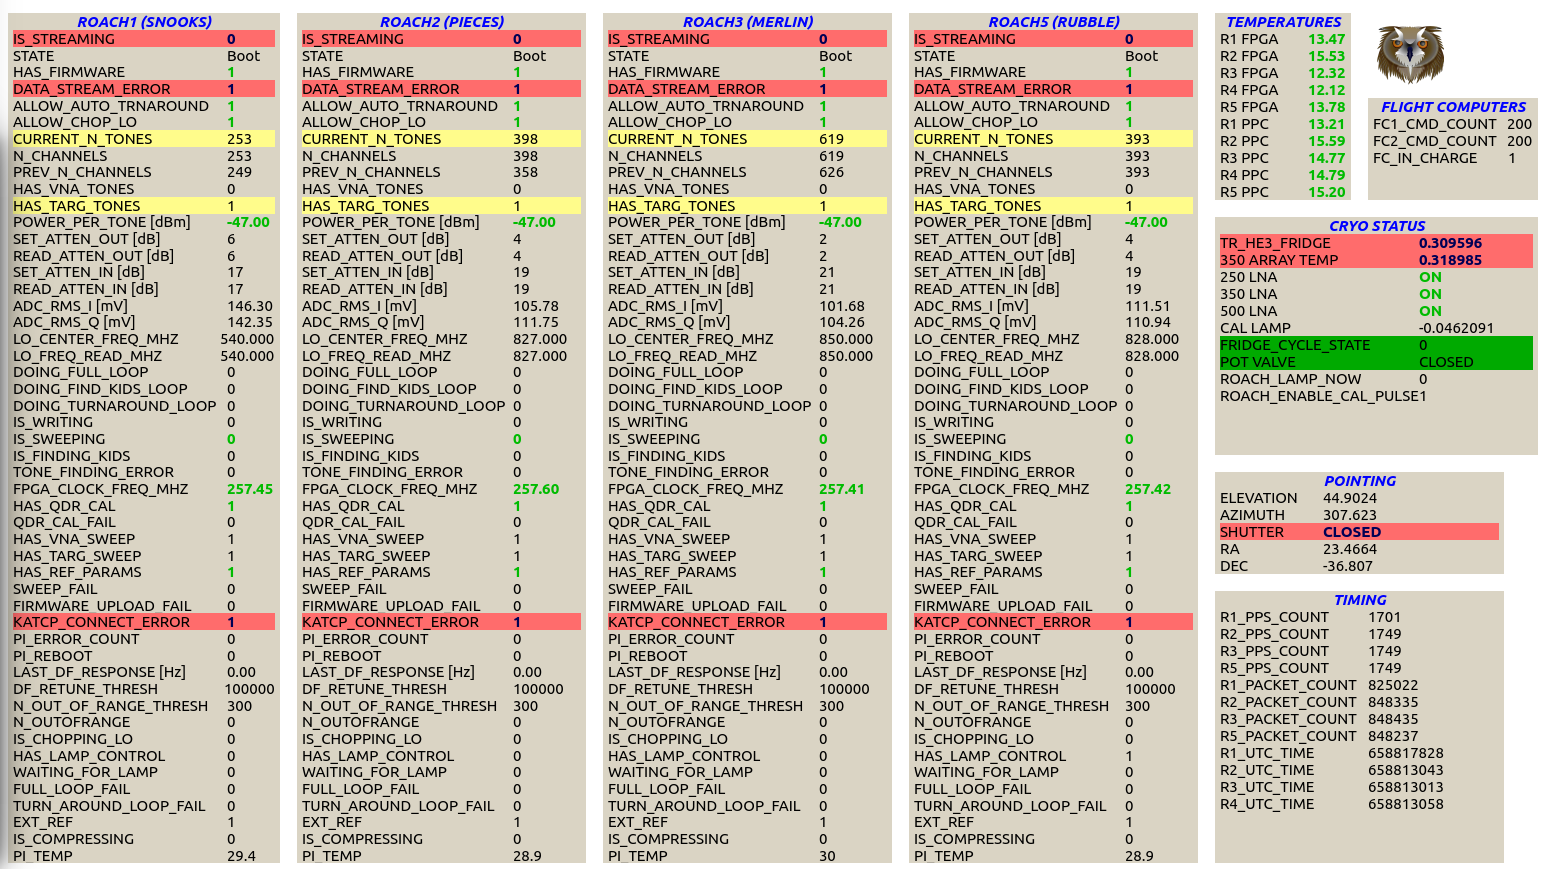
\includegraphics[angle=90, width=\linewidth,height=\textheight,keepaspectratio]{./figures/software/roaches_off}
\caption{\texttt{Owl} screen when the ROACHs are powered down.}
\label{fig:roaches off screen}
\end{figure}

\begin{figure}[hbtp]
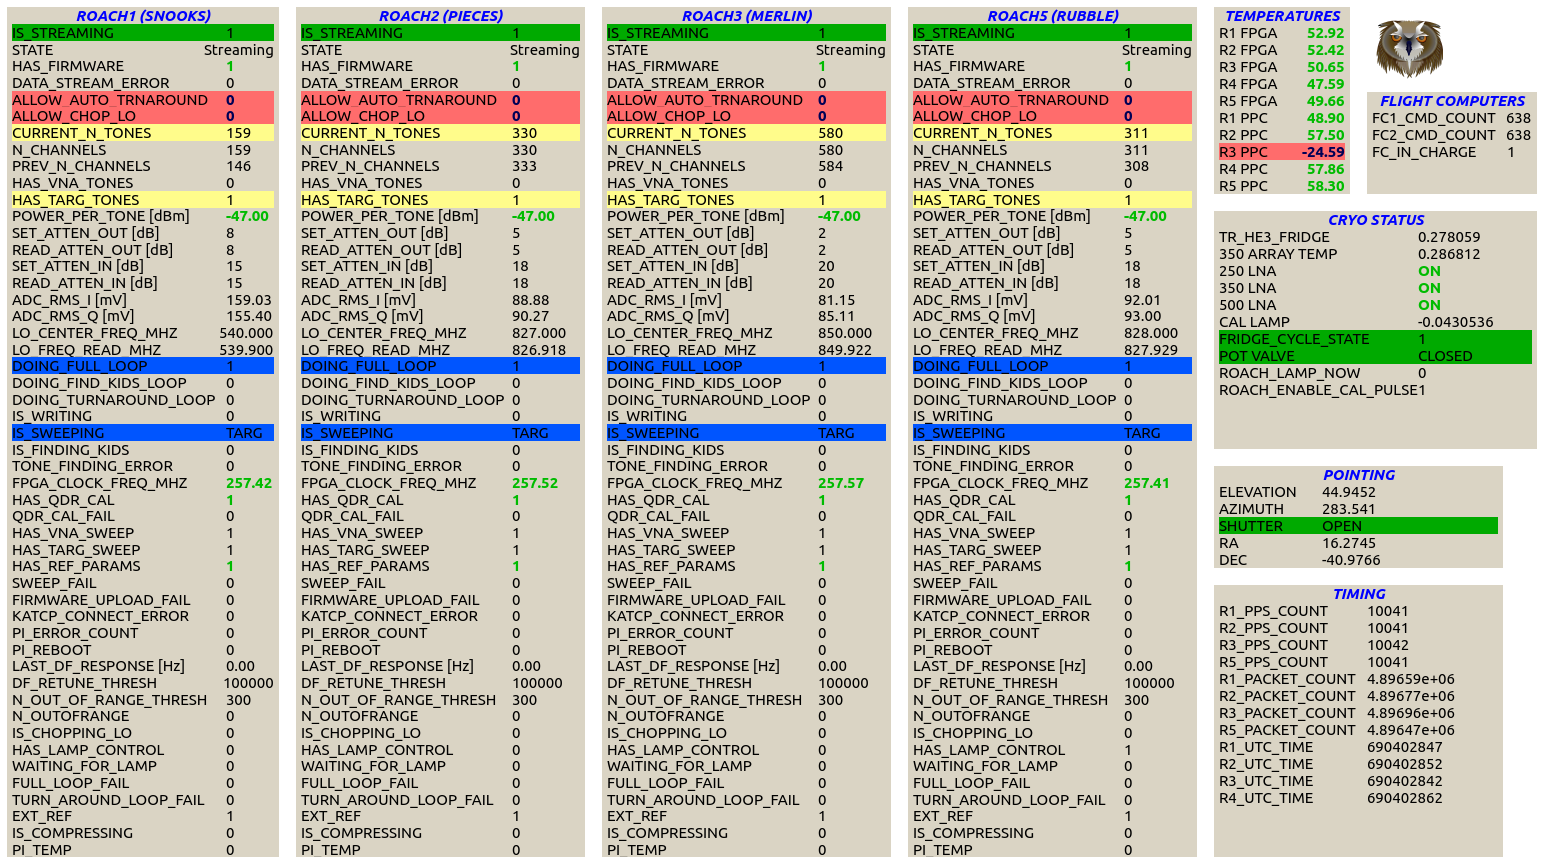
\includegraphics[angle=90, width=\linewidth,height=\textheight,keepaspectratio]{./figures/software/full_loop}
\caption{\texttt{Owl} screen when the ROACHs are performing a full loop.}
\label{fig:doing full loop screen}
\end{figure}

\begin{figure}[hbtp]
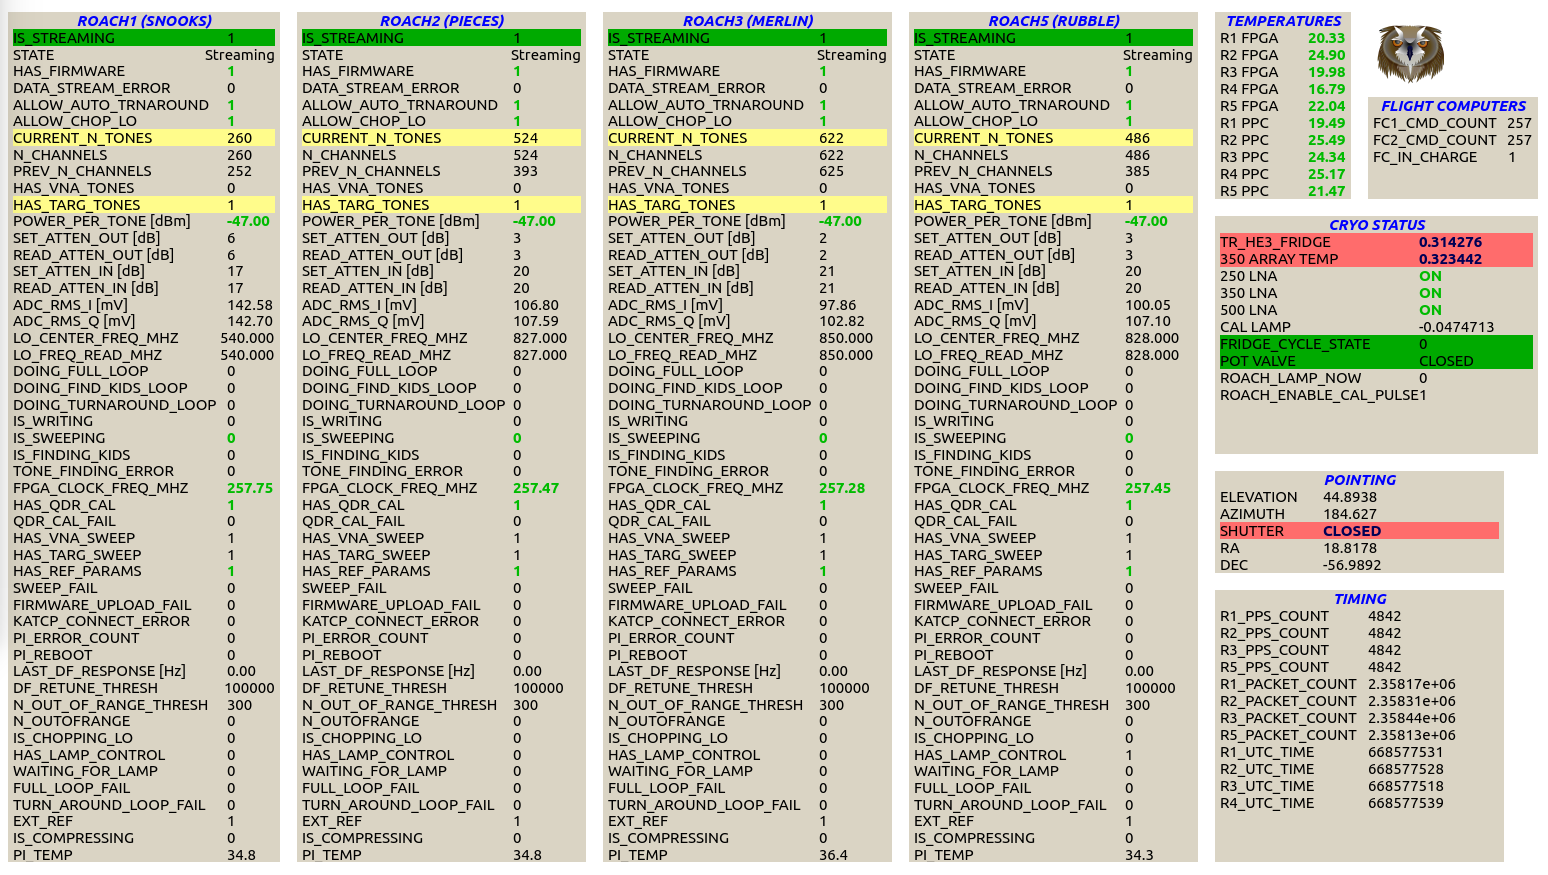
\includegraphics[angle=90, width=\linewidth,height=\textheight,keepaspectratio]{./figures/software/has_targ_tones}
\caption{\texttt{Owl} screen when the ROACHs are streaming, with target tones.}
\label{fig:has targ tones screen}
\end{figure}

\section{Commands}
The following is a description of the core set of commands which can be used to control the readout during normal lab, or flight operation. Syntax is given for manually inputting them into \texttt{blastcmd}, although during flight they will most likely be executed using \texttt{Cow}.
$^{*}$CAUTION--- don’t execute these commands unless you have a plan in mind.
$^{**}$EXTRA CAUTION- improper use of these commands will lead to a decrease in the number of future BLAST-TNG science publications. If you think you might need to use one, first try to contact SG or AS.
Note:\\
$<$which roach$>$ is an integer in (1,5).
Commands which execute sequences of events:

\begin{itemize}[leftmargin=*,label={}]

\item \textbf{full\_loop}: Triggers a full-loop. See: Multi-command loops.
Arguments:
\begin{itemize}
  \item Which ROACH (1-5)
  \item KID-finding mode (see: KID-finding)
    1 = default
    2 = use configurable parameters
  \item Target power/tone, in dBm (-47 dBm typical for full-loop).
\end{itemize}

Syntax: \texttt{full\_loop <which roach> <KID-finding mode> <power/tone in dBm>}

\item \textbf{full\_loop\_all}: Triggers a full-loop for all ROACHs. See: Multi-command loops.
Arguments: See \texttt{full\_loop}

Syntax: \texttt{full\_loop\_all <KID-finding mode <power/tone in dBm>}

\item \textbf{full\_loop\_default}: Triggers a full-loop for all ROACHs, using previously chosen KID-finding mode and power/tone. See: Multi-command loops, \texttt{full\_loop}, \texttt{full\_loop\_all}.

Syntax: \texttt{full\_loop\_default}, \texttt{full\_loop\_default\_all}

\item \textbf{turnaround\_loop}: Triggers an elevation turnaround loop for a single ROACH. See: Normal operation.
Arguments:
\begin{itemize}
  \item Which ROACH (1-5)
  \item KID-finding mode (see: KID-finding)
    1 = Default
    2 = Use configurable parameters
  \item Target power/tone, in dBm (-47 dBm typical).
\end{itemize}

Syntax: \texttt{turnaround\_loop <which roach> <KID-finding mode> <power/tone in dBm>}

\item \textbf{turnaround\_loop\_all}: Triggers an elevation turnaround loop for all ROACHs. See: Multi-command loops.
Arguments: See \texttt{turnaround\_loop}

Syntax: \texttt{turnaround\_loop\_all <KID-finding mode> <power/tone in dBm>}

\item \textbf{find\_kids\_loop}: Triggers the find-kids-loop for a single ROACH.
Arguments:
\begin{itemize}
  \item Which ROACH (1-5)
  \item KID-finding mode (see: KID-finding)
    1 = Default
    2 = Use configurable parameters
  \item Target power/tone, in dBm (-47 dBm typical).
  \end{itemize}

Syntax: \texttt{find\_kids\_loop $<$which roach$>$}

\item \textbf{find\_kids\_loop\_all}: Triggers the find-kids-loop for all ROACHs.
Arguments: See \texttt{find\_kids\_loop}

Syntax: \texttt{find\_kids\_loop\_all <KID-finding mode> <power/tone in dBm>}

\item \textbf{refit\_freqs}: Does a target sweep, calculates the $\Delta$f between carrier and resonant frequencies, adjusts the tone frequencies, and re-sweeps to store a new reference sweep and set of reference parameters.

Syntax: \texttt{refit\_freqs <which roach> 1}

\item \textbf{refit\_freqs\_all}: As above, for all ROACHs.

Syntax: \texttt{refit\_freqs\_all}

\end{itemize}

\subsection{Commands which are useful for data visualization (KST)}
Commands which are useful for data visualization (KST):

\begin{itemize}[leftmargin=*,label={}]

\item \textbf{zero\_df\_all}: Calculates (for all ROACHs) the mean $\Delta$f value from the last 50 values, and subtracts it from all future $\Delta$f values. This centers the $\Delta$f timestreams around DC, which is useful for measuring frequency drift as function of time in the KST detector timestreams (see: \texttt{Mole}).

Syntax: \texttt{zero\_dfs}

\end{itemize}

\subsection{Commands that enable triggering of periodic events}

\begin{itemize}[leftmargin=*,label={}]

\item \textbf{enable\_chop\_lo\_all}: If set high, allows the LO to perform a three-point frequency chop at azimuth turnarounds.

Syntax: \texttt{enable\_chop\_lo\_all <0\textbar 1>}

\item \textbf{roach\_allow\_scan\_check}: Enables the automatic elevation turnaround-loop for a single ROACH.

\item \textbf{roach\_allow\_scan\_check\_all}: Enables the automatic elevation turnaround-loop for all ROACHs.

Syntax: \texttt{roach\_allow\_scan\_check\_all}

\item \textbf{roach\_disallow\_scan\_check}: Disables the automatic elevation turnaround-loop for a single ROACH.

Syntax: \texttt{roach\_disallow\_scan\_check <which roach>}

\item \textbf{roach\_disallow\_scan\_check\_all}: Disables the automatic elevation turnaround-loop for all ROACHs.

Syntax: \texttt{roach\_disallow\_scan\_check\_all}

\end{itemize}

\subsection{Tone writing commands}
\begin{itemize}[leftmargin=*,label={}]

\item $^{*}$\textbf{reload\_vna\_all}: Loads/reloads the VNA comb to all ROACHs. Use only when debugging.

Syntax: \texttt{reload\_vna\_all}

\item $^{*}$\textbf{load\_freqs}: Loads the last set of target frequencies which was found during channel assignment. Frequencies are read from the file \texttt{bb\_target\_freqs.dat}, stored in the root directory of each ROACH.

Syntax: \texttt{load\_freqs <which roach>}

\item $^{*}$\textbf{load\_freqs\_all}: Same as above, for all ROACHs.

Syntax: \texttt{load\_freqs\_all}

\end{itemize}

\subsection{LO commands}

\begin{itemize}[leftmargin=*,label={}]

\item \textbf{center\_lo}: Sets the LO frequency for a single Valon to its nominal center frequency (hard-coded in \texttt{roach.c}).

Syntax: \texttt{center\_lo <which roach>}

\item \textbf{center\_lo\_all}: Same as \texttt{center\_lo}, but for all ROACHs.

Syntax: \texttt{center\_lo\_all}

\item \textbf{chop\_lo}: See: Housekeeping/automatic. Does a three-point LO frequency chop about the LO center frequency.

Syntax: \texttt{chop\_lo $<$which roach$>$}
For the command to execute, the following conditions must be true:

\begin{enumerate}
\item \texttt{ALLOW\_AUTO\_CHOP} = 1 (see \texttt{enable\_chop\_lo})
\item \texttt{ALLOW\_AUTO\_TURNAROUND} = 0 (see \texttt{roach\_allow\_scan\_check})
\item \texttt{IS\_SWEEPING} = 0
\end{enumerate}

\item$^{*}$\textbf{offset\_lo}: Offsets the LO frequency by specified amount in Hz, relative to center frequency.\

Syntax: \texttt{offset\_lo <which roach> <some number of Hz (can be <0)>}\\
Note: If you offset Roach1’s LO by 1000 Hz, e.g.,
\begin{verbatim}
> offset_lo 1 1000
\end{verbatim}
and then decide that you actually wanted to offset it by 2000 Hz, there is no need to recenter the LO. Just do:
\begin{verbatim}
> offset_lo 1 2000
\end{verbatim}
The LO frequency will now be +2000 Hz above its center frequency. However, before resuming normal operation, you must manually recenter the LO, by using the \texttt{center\_lo} command.

\item $^{*}$\textbf{offset\_lo\_all}: Same as \texttt{offset\_lo}, but for all ROACHs.

Syntax: \texttt{offset\_lo\_all}

\item \textbf{recenter\_lo}: Returns the LO frequency to the default center frequency (hard-coded for each ROACH in \texttt{roach.c}).

Syntax: \texttt{recenter\_lo <which roach>}

\item \textbf{recenter\_lo\_all}: Same as \texttt{recenter\_lo}, but for all ROACHs.

Syntax: \texttt{recenter\_lo\_all}

\item \textbf{read\_lo}: Read the current LO frequency. Frequency is returned in MHz.

Syntax: \texttt{read\_lo <which roach>}

\item \textbf{set\_lo\_MHz}: Set the current LO frequency, in MHz.

Syntax: \texttt{set\_lo\_MHz <which roach>}

\end{itemize}

\subsection{Tone power/attenuator commands}
\begin{itemize}[leftmargin=*,label={}]

\item \textbf{read\_attens}: Reads the current attenuator settings. The result, in dB, will appear in the Owl fields: \texttt{READ\_ATTEN\_OUT}, \texttt{READ\_ATTEN\_IN}.

Syntax: \texttt{read\_attens <which roach>}

\item \textbf{show\_adc\_rms}: Reads the current root-mean-square voltage level of the signals at the input to the ADCs (I and Q), in millivolts. The values are displayed in the \texttt{ADC\_RMS\_I} and \texttt{ADC\_RMS\_Q} Owl fields.

Syntax: \texttt{show\_adc\_rms <which roach>}

\item \textbf{set\_attens}: Set the RUDATs for a single ROACH, in dB. The requested values will appear in the Owl fields: \texttt{SET\_ATTEN\_OUT}, \texttt{SET\_ATTEN\_IN}.

Syntax: \texttt{set\_attens <which roach> <float output atten, dB> <float input atten, dB>}

\item \textbf{set\_attens\_default}: Sets the RUDATs to their default values, which are defined in roach.c as 4 db (output), 19 dB (input). The requested values will appear in the Owl fields: \texttt{SET\_ATTEN\_OUT}, \texttt{SET\_ATTEN\_IN}.

Syntax: \texttt{set\_attens\_default <which roach>}

\item \textbf{set\_attens\_default\_all}: Same as above, or all ROACHs. The set values will appear in the Owl fields: \texttt{SET\_ATTEN\_OUT}, \texttt{SET\_ATTEN\_IN}.

\item \textbf{set\_attens\_calc}: Automatically set the output attenuator to target a power/tone, in dBm. The calculated power level takes into account the current number of tones. The input attenuator value is chosen to enforce a total attenuation of 23 dB between the input and output. The default is -47 dBm/tone. The set values will appear in the Owl fields: \texttt{SET\_ATTEN\_OUT}, \texttt{SET\_ATTEN\_IN}.

Syntax: \texttt{set\_attens\_calc <which roach> <float power/tone, in dBm>}

\item \textbf{set\_attens\_last\_all}: Sets the input and output attenuators to their last set values. These values are read from the file: \texttt{last\_attens.dat}, located on FC1/FC2 in: \texttt{~/roach\_flight/roach<which roach>}
The set values will appear in the Owl fields: \texttt{SET\_ATTEN\_OUT}, \texttt{SET\_ATTEN\_IN}.

Syntax: \texttt{set\_attens\_last\_all <float output atten, dB> <float input atten, dB>}

\item $^{**}$\textbf{set\_attens\_min\_output}: Sets the output attenuators of all ROACHs to 30 dB. This mode is used to measure the warm electronics noise contribution to the total noise budget. It’s flagged because it would be bad to set this and then forget to revert back to normal settings. The set values will appear in the \texttt{Ow} fields: \texttt{SET\_ATTEN\_OUT}, \texttt{SET\_ATTEN\_IN}.

Syntax: \texttt{set\_attens\_min\_output\_all}

\item \textbf{set\_attens\_conserved}: Sets the output attenuator to specified number of dB, while choosing the input attenuator level to conserve a total of 23 dB between the pair. The set values will appear in the \texttt{Owl} fields: \texttt{SET\_ATTEN\_OUT}, \texttt{SET\_ATTEN\_IN}.

Syntax: \texttt{set\_attens\_conserved <which roach> <float output atten, dB>}

\end{itemize}

\subsection{Pi commands}
\begin{itemize}[leftmargin=*,label={}]

\item $^{*}$\textbf{reboot\_pi}: Reboots the specified Pi, by sending \texttt{sudo reboot} to the netcat server listening on ports 12345 or 12346.

Syntax: \texttt{reboot\_pi <which roach> <PORT\#>}
Note: MCP will automatically reboot a Pi after 10 errors are registered by the Valon and/or attenuator clients. This command should only be used in the event that automatic rebooting appears to have failed. If the Pi is already powered down, the command will have no effect. If needed, verify that the Pi is powered up by pinging it at the IP address specified in the Hardware Addresses section. After rebooting, the Valon and attenuator servers start up automatically (they are in \texttt{/etc/rc.local} on the Pis). There is no need to manually configure anything after reboot.

\item $^{**}$\textbf{roach\_set\_extref}: Configure the Valons to use either the external (1, default for flight-mode) or internal (0) PLL reference.

Syntax: \texttt{roach\_set\_extref <which roach> < 0 | 1 >}
Note: By default, the Valon uses the external 10 MHz reference signal provided by the OctoClock. If the external reference signal drops out or changes frequency, the LO and FPGA clock signals generated by the Valon will become unstable and/or drop out entirely. This command is intended for use only in this scenario. Signs that the external reference has dropped out may include:
\begin{itemize}
  \item Accompanied loss of PPS signal (check PPS counter fields in \texttt{Owl}).
  \item Nonsensical channel data lasting for more than a few seconds.
  \item No channel timestreams at all (flat line, possibly with a DC offset).
\end{itemize}
The clearest indication that the external reference has dropped out will be a QDR RAM calibration fail after resetting the ROACHs, with an out-of-range FPGA clock frequency reported by Owl (see \texttt{FPGA\_CLOCK\_FREQ} field).

If you have no other option but to use this command, follow this procedure:
\begin{enumerate}
  \item Send the command to switch one or more (see \textit{all} version) to internal reference:
\begin{verbatim}
  > roach_set_extref <which roach> 0
\end{verbatim}
  \item Power cycle the readout (see: Power commands)
\end{enumerate}

\item \textbf{read\_pi\_temps}: Read the temperatures of all Pi CPUs. The temperatures will appear in the \texttt{PI\_TEMP} field in \texttt{Owl} for each ROACH.

\end{itemize}

\subsection{Power state commands}
\begin{itemize}[leftmargin=*,label={}]

\item $^{**}$\textbf{roach\_cycle}: Power cycles all five ROACH slices.

Syntax: \texttt{roach\_cycle}

\item $^{**}$\textbf{roaches\_off}: Powers down all five ROACH slices.

Syntax: \texttt{roaches\_off}

\item \textbf{roaches\_on}: Powers up all five ROACH slices.

Syntax: \texttt{roaches\_on}

\item $^{**}$\textbf{kill\_roach}: Halts a ROACH’s PPC. The ROACH may be brought back online by power cycling the entire readout stack.

Syntax: \texttt{kill\_roach <which roach>}

\subsection{Cal lamp commands}

\item \textbf{roach\_has\_lamp\_control}: Gives exclusive control of the cal lamp to the ROACH. No other ROACHs will be able to trigger the pulse.

Syntax: \texttt{roach\_has\_lamp\_control <which roach>}

\subsection{Commands that set global parameters}
\begin{itemize}[leftmargin=*,label={}]

\item $^{*}$\textbf{set\_find\_kids\_params}: Set the KID-finding parameters. On system start-up, these parameters are automatically set to default values. See: KID-finding
Arguments:
\begin{itemize}
  \item Which ROACH (1-5)
  \item Smoothing scale (kHz, 1000.0--100000.0)
  \item Dip-depth threshold (dB, 0.1, 100)
  \item Spacing threshold (kHz, 80.0, 10000.0)
\end{itemize}

Syntax: \texttt{set\_find\_kids\_params <which roach> <smoothing scale> <dip-depth threshold> <spacing threshold>}

\item $^{*}$\textbf{set\_max\_nkids}: Sets the maximum number of channels that can be found from a VNA sweep without triggering an error. The maximum number of channels should be 500--800. See: KID-finding, \texttt{TONE\_FINDING\_ERROR}.

Syntax: \texttt{set\_max\_nkids <which roach> <max nkids>}

\item $^{*}$\textbf{set\_max\_nkids\_all}: As above, for all ROACHs.

Syntax: \texttt{set\_max\_nkids <max nkids>}

\item $^{*}$\textbf{set\_min\_nkids}: Sets the minimum number of channels that can be found from a VNA sweep without triggering an error. The minimum number of channels should be 1--50. See: KID-finding, \texttt{TONE\_FINDING\_ERROR}.

Syntax: \texttt{set\_min\_nkids <which roach> <min nkids>}

\item $^{*}$\textbf{set\_min\_nkids\_all}: As above, for all ROACHs.

Syntax: \texttt{set\_min\_nkids\_all <min nkids>}

\item \textbf{set\_df\_diff\_retune\_threshold}: See \texttt{DF\_RETUNE\_THRESH}. Sets the threshold for the cal lamp df response (df\_lamp\_on - df\_lamp\_off), in Hz.

Syntax: \texttt{set\_df\_diff\_retune\_threshold <which roach> <Hz>}

\item \textbf{set\_df\_diff\_retune\_threshold\_all}: As above, for all ROACHs.

Syntax: \texttt{set\_df\_diff\_retune\_threshold\_all <Hz>}

\item \textbf{set\_n\_outofrange\_thresh}: See \texttt{N\_OUTOFRANGE\_THRESH}. Sets the threshold for number of channels which can be out of range (df lamp response).

Syntax: \texttt{set\_n\_outofrange\_thresh <which roach> <number of chan>}

\item \textbf{set\_n\_outofrange\_thresh\_all}: As above, for all ROACHs.

Syntax: \texttt{set\_n\_outofrange\_thresh <number of chan>}

\item \textbf{set\_default\_tone\_power}: Sets the default power/tone (dBm) used by \texttt{full\_loop\_default}. Typical power/tone is -47 dBm.

Syntax: \texttt{set\_default\_tone\_power <which roach> <power/tone, in dBm>}

\item \textbf{set\_default\_tone\_power\_all}: As above, for all ROACHs.

Syntax: \texttt{set\_default\_tone\_power\_all <power/tone, in dBm>}

\end{itemize}

\subsection{Data handling commands}
\begin{itemize}[leftmargin=*,label={}]
  \item
\end{itemize}
\item \textbf{compress\_roach\_data}: Compresses the most recent set of the specified data type for each ROACH slice into a single tar.gz. Each tarball is assigned a local environment variables based on its data type, which should be specified as the file path when downlinking data.

Syntax: \texttt{compress\_roach\_data <0-6>}
where:
0 = VNA sweeps
1 = Target sweeps
2 = IQ timestreams
3 = DF timestreams
4 = Lamp responses ($\Delta$f, I, Q)
5 = Noise comparison data
6 = Baseband target frequency lists
Environment variables:
0 = \$ALL\_VNA\_SWEEPS
1 = \$ALL\_TARG\_SWEEPS
2 = \$ALL\_IQ\_DATA
3 = \$ALL\_DF\_DATA
4 = \$ALL\_LAMP\_DATA
5 = \$ALL\_NOISE\_COMP
6 = \$ALL\_BB\_FREQS

\end{itemize}

\section{Data downlinking}

Several commands result in data being saved on FC1/FC2. Some of the data is overwritten each time it’s created (e.g., the lamp responses in $\Delta$f, I, and Q (\texttt{lamp\_response.dat}). Other data (e.g., the VNA and target sweep data) is time-stamped and stored on the hard drives as a record of the flight. When data which would be useful to view during the flight is created, MCP automatically creates a tarball of the data for each ROACH, which is overwritten with each consecutive data creation. These tarballs are given unique environment variables corresponding to their data type. These environment variables can be input into \texttt{Cow} to downlink the data. The variables are:

\begin{itemize}[leftmargin=*,label={}]

\item \texttt{\$R<1-5>\_LAST\_VNA\_SWEEP}
\item \texttt{\$R<1-5>\_LAST\_TARG\_SWEEP}
\item \texttt{\$R<1-5>\_LAST\_DF\_DATA}
\item \texttt{\$R<1-5>\_LAST\_IQ\_DATA}
\item \texttt{\$R<1-5>\_LAST\_LAMP\_DATA}
\item \texttt{\$R<1-5>\_LAST\_BB\_TARG\_FREQS}
\item \texttt{\$R<1-5>\_LAST\_TARG\_FREQS\_MAGS}
\item \texttt{\$R<1-5>\_LAST\_NOISE\_COMP}

\item \textbf{Example I}: Getting data for all ROACHs
To downlink a tarball containing all the most recent VNA sweeps for each ROACH, from \texttt{Cow}:
\begin{enumerate}
  \item In ROACH commands: \texttt{compress\_roach\_data 0}
  \item Go to Telemetry screen
  \item Choose: \texttt{Request\_stream\_file}
    Choose options:
    Downlink =
    Fragment \# = 0
    File block number = 1
    Absolute file path = \texttt{\$ALL\_VNA\_SWEEPS}
  \item On GROUNDSTATION-1, go to: \texttt{/data/etc/downloaded\_files}
  \item The downlinked file will appear as: \texttt{file\_block\_1}
  \item A bash script (\texttt{untarloop.sh}) running in the background will untar the file when downlink is complete, and move the data to the appropriate directories.
\end{enumerate}

\item \textbf{Example II}: Getting data for a single ROACH
To downlink a VNA sweep tarball containing data for a single ROACH, \texttt{Cow}:
\begin{enumerate}
  \item Go to Telemetry screen
  \item Choose: \texttt{Request\_stream\_file}
    Choose options:
    Downlink =
    Fragment \# = 0
    File block number = 1
    Absolute file path = \texttt{\$R1\_LAST\_VNA\_SWEEP}
  \item On GROUNDSTATION-1, go to: \texttt{/data/etc/downloaded\_files}
  \item The downlinked file will appear as: \texttt{file\_block\_1}
  \item A bash script (\texttt{untarloop.sh}) running in the background will untar the file when downlink is complete, and move the data to the appropriate directories.
\end{enumerate}

\end{itemize}
